\documentclass[10pt]{article}
\usepackage{times}
\usepackage{geometry}
\usepackage{multicol}
\usepackage{setspace}
\usepackage{parskip} 
\usepackage{booktabs} 
\usepackage{caption}
\usepackage{graphicx}
\usepackage{float}
\usepackage{fancyhdr}   
\usepackage{array}
\usepackage{amsmath} 
\usepackage{booktabs}
\usepackage{hhline}
\usepackage{multirow}
\usepackage[hidelinks]{hyperref}
\usepackage{pdflscape} % Tambahkan package untuk landscape
\bibliographystyle{ieeetr}

% Configure table caption style
\captionsetup[table]{font=small,skip=3pt}
\renewcommand{\tablename}{Tabel}

% Configure figure caption style
\captionsetup[figure]{font=small,justification=centering,skip=3pt}
\renewcommand{\figurename}{Gambar}

% Configure footer
\pagestyle{fancy}
\fancyhf{}
\fancyfoot[C]{\rule{\textwidth}{0.4pt}\\ \thepage} % Tambahkan nomor halaman

\makeatletter
\renewcommand\section{\@startsection{section}{1}{\z@}%
  {-3.5ex \@plus -1ex \@minus -.2ex}%
  {2.3ex \@plus.2ex}%
  {\normalfont\normalsize\bfseries}}
\renewcommand\subsection{\@startsection{subsection}{2}{\z@}%
  {-3.25ex\@plus -1ex \@minus -.2ex}%
  {1.5ex \@plus .2ex}%
  {\normalfont\itshape\normalsize}}
\renewcommand\subsubsection{\@startsection{subsubsection}{3}{\z@}%
  {-3.25ex\@plus -1ex \@minus -.2ex}%
  {1.5ex \@plus .2ex}%
  {\normalfont\itshape\normalsize}}
\makeatother

\geometry{
    a4paper,
    left=25mm,
    right=25mm,
    top=25mm,
    bottom=25mm
}

\setstretch{1.0} % Single spacing
\setlength{\parskip}{6pt} % Set spacing between paragraphs

\renewcommand{\thesection}{\arabic{section}.}
\renewcommand{\thesubsection}{\arabic{section}.\arabic{subsection}}

\begin{document}
{\fontsize{15}{18}\selectfont
\begin{center}
    Stroke Prediction using Machine Learning
\end{center}}

\begin{center}
    {\fontsize{10}{12}\selectfont Yusra Erlangga Putra$^1$, Sheryl Anastasya$^{2}$, Resky Auliyah Kartini Askin$^3$, Ivan Betrandi$^4$, Amaliah Diah$^5$}\\
    {\fontsize{9}{11}\selectfont
    \begin{tabular}{c}
        Departemen Matematika, Fakultas Matematika dan Ilmu Pengetahuan Alam, Universitas Hasanuddin, Makassar, Indonesia \\
        $^1$yusraerlangg@gmail.com, $^{2}$sherylanastasya2809@gmail.com                                                   \\
    \end{tabular}}
\end{center}

\vspace{0.5cm}

{\fontsize{10}{12}\selectfont\noindent\textbf{\textit{Abstrak}}}

\noindent{\fontsize{9}{11}\selectfont\itshape%
    Stroke adalah penyebab utama kecacatan jangka panjang dan kematian di seluruh dunia, dengan risiko yang meningkat seiring bertambahnya usia serta adanya faktor risiko seperti hipertensi dan diabetes. Tujuan penelitian ini adalah mengembangkan model prediksi dini yang akurat untuk stroke sehingga memungkinkan intervensi perawatan kesehatan preventif yang efektif. Penelitian ini menggunakan algoritma Random Forest dan Support Vector Machine (SVM). Karena ketidakseimbangan pada himpunan data, teknik Synthetic Minority Oversampling Technique (SMOTE) diterapkan untuk meningkatkan representasi data minoritas. Model dioptimalkan melalui penyesuaian hiperparameter menggunakan Optimasi Bayesian. Evaluasi model dilakukan dengan metrik akurasi, presisi, sensitivitas, dan skor-F1, menggunakan validasi silang K-Fold yang dimodifikasi untuk memastikan keandalan pada data yang belum terlihat. Hasil eksperimen menunjukkan bahwa algoritma SVM dengan SMOTE dan Optimasi Bayesian mencapai akurasi tertinggi. Temuan ini menunjukkan bahwa model \textit{machine learning} yang dioptimalkan dapat memberikan kontribusi signifikan dalam prediksi dini stroke dan mendukung pengambilan keputusan dalam sistem perawatan kesehatan preventif.
    \par}

\noindent{\fontsize{9}{11}\selectfont
    \textit{\textbf{Kata kunci:} Prediksi Stroke, \textit{machine learning}, Random Forest, Support Vector Machine, SMOTE, Bayesian Optimization}
    \par}

\begin{multicols}{2}
    \setlength{\columnsep}{0.4pt} %
    \raggedcolumns%
    \sloppy

    \section{Introduction}
    \subsection{Background}
    Stroke merupakan masalah kesehatan global yang serius, menempati posisi kedua
    sebagai penyebab kematian tertinggi dan posisi ketiga sebagai penyebab
    kecacatan di dunia. Menurut data WHO, satu dari empat orang berisiko mengalami
    stroke dalam masa hidupnya, dengan 70\% kasus terjadi di negara-negara
    berpenghasilan rendah dan menengah\cite{who2024stroke}. Di Indonesia sendiri,
    angka kejadian stroke mencapai 10,9 per 1000 penduduk, dengan sekitar 137 orang
    per 100.000 penduduk meninggal akibat stroke setiap
    tahunnya\cite{kemenkes2023stroke}. Beban ekonomi yang ditimbulkan stroke juga
    sangat besar, mencakup biaya perawatan medis langsung dan hilangnya
    produktivitas akibat kecacatan jangka panjang.

    Kompleksitas faktor risiko stroke yang meliputi tekanan darah tinggi,
    kolesterol, diabetes, obesitas, dan gaya hidup, menjadikan prediksi stroke
    sebagai tantangan yang signifikan dalam dunia kesehatan\cite{boehme2017stroke}.
    Namun, deteksi dini risiko stroke memiliki potensi besar dalam mencegah
    kejadian stroke dan menurunkan tingkat kematian serta kecacatan. Studi
    menunjukkan bahwa hingga 80\% kasus stroke dapat dicegah melalui manajemen
    faktor risiko yang tepat\cite{strokepreventionstudy2022}. Oleh karena itu,
    pengembangan sistem prediksi stroke yang akurat menjadi sangat penting dalam
    upaya pencegahan.

    Prediksi dini stroke menggunakan metode konvensional seringkali terbatas dalam
    kemampuannya mengintegrasikan berbagai faktor risiko secara simultan.
    Perkembangan \textit{machine learning} membuka peluang baru dalam meningkatkan
    akurasi prediksi stroke. Dengan kemampuannya menganalisis data kompleks dalam
    jumlah besar, teknik \textit{machine learning} dapat mengidentifikasi pola-pola
    tersembunyi dan korelasi antar berbagai faktor risiko yang sulit dideteksi
    melalui metode konvensional.

    Penelitian ini mengusulkan pendekatan inovatif dengan algoritma Random Forest
    dan Support Vector Machine (SVM) untuk prediksi stroke.\@ Kedua algoritma ini
    dipilih karena kemampuannya dalam menangani data kesehatan yang kompleks dan
    menghasilkan model prediksi yang akurat. Untuk mengatasi masalah
    ketidakseimbangan data yang umum dalam kasus medis, diterapkan teknik SMOTE
    (Synthetic Minority Oversampling Technique). Selanjutnya, optimasi Bayesian
    digunakan untuk meningkatkan performa model melalui penyetelan hiperparameter
    yang optimal. Pendekatan komprehensif ini diharapkan dapat menghasilkan sistem
    prediksi stroke yang lebih andal dan aplikatif dalam praktik klinis.

    \subsection{Literature Review}
    % Brief review of related research goes here...

    \subsection{Research Rationale}
    Penelitian ini didasari oleh beberapa pertimbangan penting dalam konteks
    prediksi stroke menggunakan \textit{machine learning}. Pertama, meskipun telah
    banyak penelitian yang menggunakan berbagai algoritma seperti Logistic
    Regression\cite{guhdar2023optimizing}, Decision Tree, dan Neural
    Network\cite{dev2022predictive}, masih terdapat tantangan dalam menangani
    ketidakseimbangan data pada kasus medis. Ketidakseimbangan ini dapat
    menyebabkan bias dalam model prediksi yang berpotensi menghasilkan kesalahan
    diagnosis serius dalam praktik klinis.

    Kedua, penelitian-penelitian sebelumnya\cite{yang2021accurate,
        zhi2024exploration, azam2020performance} cenderung berfokus pada penggunaan
    algoritma tunggal tanpa mempertimbangkan optimasi parameter secara sistematis.
    Pendekatan tersebut berpotensi menghasilkan model yang suboptimal. Oleh karena
    itu, penelitian ini mengusulkan integrasi teknik Optimasi Bayesian untuk
    mengoptimalkan parameter model.

    \subsection{Research Questions and Objectives}
    Berdasarkan pertimbangan tersebut, penelitian ini bertujuan menjawab beberapa
    pertanyaan kunci: (1) bagaimana perbandingan efektivitas Random Forest dan SVM
    linear dalam memprediksi risiko stroke?, (2) seberapa signifikan pengaruh
    optimasi parameter menggunakan Optimasi Bayesian terhadap performa model?, dan
    (3) bagaimana dampak penerapan teknik SMOTE terhadap kinerja prediksi pada data
    yang tidak seimbang?

    Untuk menjawab pertanyaan-pertanyaan tersebut, penelitian ini memiliki tiga
    sasaran utama:
    \begin{enumerate}
        \item Mengembangkan dan membandingkan model prediksi stroke menggunakan Random Forest
              dan SVM linear
        \item Mengoptimalkan parameter model menggunakan Optimasi Bayesian untuk meningkatkan
              akurasi prediksi
        \item Mengevaluasi efektivitas teknik SMOTE dalam menangani ketidakseimbangan data
              medis
    \end{enumerate}

    Hasil penelitian ini diharapkan dapat memberikan kontribusi dalam pengembangan
    sistem pendukung keputusan klinis untuk deteksi dini risiko stroke.

    \section{Research Methods}
    \subsection{Dataset Description}
    Dataset yang digunakan dalam penelitian ini berasal dari \textit{Kaggle Stroke
        Prediction Dataset}\cite{kaggleStrokePredictionDataset}, yang berisi informasi
    kesehatan dari 5110 pasien dan memiliki 12 variabel. Dataset ini mencakup
    berbagai parameter demografis dan faktor risiko kesehatan yang berpotensi
    terkait dengan kejadian stroke. Data dikumpulkan dari berbagai fasilitas
    kesehatan dan mencakup informasi seperti usia, jenis kelamin, berbagai
    penyakit, dan gaya hidup pasien. Deskripsi fitur dataset dapat dilihat pada
    Tabel \ref{tab:dataset-description}. Output kolom stroke adalah variabel target
    biner yang menunjukkan status stroke pasien, dengan nilai 1 yang berarti pasien
    pernah mengalami stroke dan nilai 0 yang berarti tidak pernah mengalami stroke.
    Dari total 5110 sampel dalam dataset, hanya terdapat 249 kasus stroke (4,87\%)
    dan 4861 kasus non-stroke (95,13\%) yang bisa dilihat pada Gambar
    \ref{fig:class-distribution}. Hal ini menunjukkan bahwa dataset memiliki
    sebaran yang sangat tidak seimbang. Ketidakseimbangan yang signifikan ini
    merupakan karakteristik umum dalam dataset medis dan menjadi tantangan khusus
    dalam pengembangan model prediksi yang akurat. Untuk mengatasi
    ketidakseimbangan tersebut, penelitian ini menerapkan teknik SMOTE untuk
    menghasilkan sampel sintetis dari kelas minoritas sehingga dapat meningkatkan
    kinerja model dalam mendeteksi kasus stroke.

    \begin{figure}[H]
        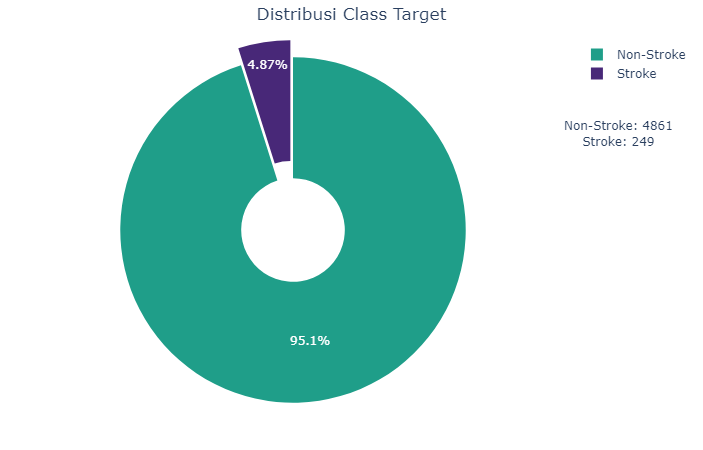
\includegraphics[width=\columnwidth]{./assets/class-distribution.png}
        \caption{Distribusi Kelas pada Dataset Stroke Prediction}%
        \label{fig:class-distribution}
    \end{figure}

    \begin{table}[H]
        \centering
        {\fontsize{8}{10}\selectfont
            \caption{Deskripsi Fitur Dataset Stroke Prediction}%
            \label{tab:dataset-description}
            \begin{tabular}{>{\raggedright\arraybackslash}p{2cm}>{\raggedright\arraybackslash}p{3cm}>{\raggedright\arraybackslash}p{1.5cm}}
                \specialrule{0.07em}{0em}{0.06em}
                \specialrule{0.07em}{0em}{0.4em}
                \textbf{Fitur}      & \textbf{Deskripsi}                                                                                                       & \textbf{Tipe Data} \\
                \midrule
                id                  & Identifier unik setiap pasien                                                                                            & Numerik            \\
                gender              & Jenis kelamin pasien (\textit{Male}, \textit{Female}, \textit{Other})                                                    & Kategorikal        \\
                age                 & Usia pasien                                                                                                              & Numerik            \\
                hypertension        & 0 jika pasien tidak memiliki hipertensi, 1 jika memiliki hipertensi                                                      & Biner              \\
                heart\_disease      & 0 jika pasien tidak memiliki penyakit jantung, 1 jika memiliki penyakit jantung                                          & Biner              \\
                ever\_married       & Status pernikahan (\textit{Yes}, \textit{No})                                                                            & Kategorikal        \\
                work\_type          & Tipe pekerjaan (\textit{children}, \textit{Govt\_job}, \textit{Never\_worked}, \textit{Private}, \textit{Self-employed}) & Kategorikal        \\
                Residence\_type     & Tipe tempat tinggal (\textit{Rural}, \textit{Urban})                                                                     & Kategorikal        \\
                avg\_glucose\_level & Level glukosa rata-rata dalam darah (\textit{Average Glucose Level})                                                     & Numerik            \\
                bmi                 & Body Mass Index                                                                                                          & Numerik            \\
                smoking\_status     & Status merokok (\textit{formerly smoked}, \textit{never smoked}, \textit{smokes}, \textit{Unknown})                      & Kategorikal        \\
                stroke              & 1 jika pasien pernah stroke, 0 jika tidak                                                                                & Biner              \\
                \bottomrule
            \end{tabular}}
    \end{table}

    \subsection{Data Preprocessing}
    Preprocessing data merupakan tahapan fundamental dalam pengembangan model
    \textit{machine learning} yang bertujuan untuk meningkatkan kualitas dan
    kesiapan data sebelum proses pemodelan. Dalam penelitian ini, preprocessing
    data dilakukan melalui empat tahapan utama: pembersihan dan penyaringan data,
    penanganan nilai yang hilang, rekayasa fitur, dan encoding variabel
    kategorikal. Setiap tahapan dirancang secara sistematis untuk mengatasi
    berbagai tantangan dalam dataset, seperti ketidaklengkapan data, variasi format
    data, dan kebutuhan standardisasi untuk pemrosesan algoritmik.

    \subsubsection{Data Cleaning and Filtering}

    Proses preprocessing data diawali dengan analisis dan pembersihan data untuk
    memastikan kualitas serta keandalan data yang akan digunakan dalam pemodelan.
    Tahap pertama adalah eliminasi kolom identifikasi (id) dari dataset. Kolom ini
    dihapus karena bersifat unik untuk setiap pasien dan tidak memiliki kontribusi
    terhadap proses prediksi stroke. Keputusan ini diambil berdasarkan prinsip
    reduksi dimensi yang bertujuan meningkatkan efisiensi komputasi tanpa
    mengurangi informasi yang bermakna dalam dataset.

    Selanjutnya, dilakukan penyaringan data berdasarkan kategori usia dewasa dengan
    membatasi subjek berusia 18 tahun ke atas. Pembatasan ini dilakukan berdasarkan
    pertimbangan epidemiologis yang menunjukkan bahwa pola dan faktor risiko stroke
    pada populasi dewasa memiliki karakteristik yang berbeda secara signifikan
    dibandingkan dengan populasi anak-anak. Sebagaimana ditunjukkan pada Gambar
    \ref{fig:age-distribution}, fokus pada populasi dewasa tidak hanya meningkatkan
    homogenitas data tetapi juga meminimalkan potensi bias dalam prediksi,
    mengingat prevalensi stroke yang secara signifikan lebih tinggi pada kelompok
    usia dewasa.

    \begin{figure}[H]
        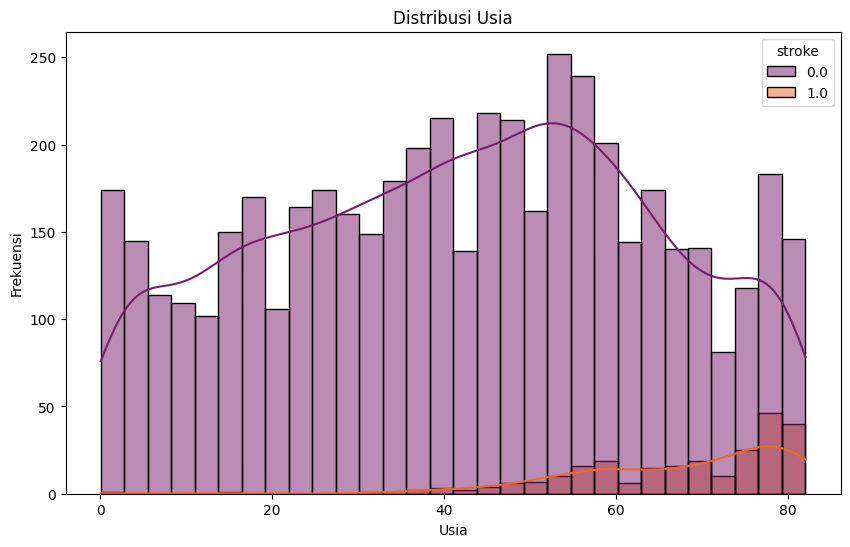
\includegraphics[width=\columnwidth]{./assets/age-distribution.png}
        \caption{Distribusi Usia pada Dataset Stroke Prediction}%
        \label{fig:age-distribution}
    \end{figure}

    \subsubsection{Handling Missing Value}

    Penanganan nilai yang hilang merupakan tahap kritis dalam proses preprocessing,
    terutama pada variabel BMI (Body Mass Index) sebagaimana tervisualisasi pada
    Gambar \ref{fig:missing-value}. Untuk mengatasi permasalahan ini, diterapkan
    metode K-Nearest Neighbors (KNN) Imputer dengan parameter
    \texttt{n\_neighbors=5}. Pemilihan metode ini didasarkan pada kemampuannya
    dalam mempertimbangkan pola dan kemiripan karakteristik antara data saat
    melakukan estimasi nilai yang hilang.

    KNN Imputer menunjukkan keunggulan dibandingkan dengan metode imputasi
    konvensional seperti mean atau median, karena kemampuannya dalam menghasilkan
    estimasi yang lebih presisi dengan mempertimbangkan konteks dan interaksi
    antarvariabel dalam dataset. Metode ini bekerja berdasarkan prinsip bahwa
    sampel-sampel dengan karakteristik serupa cenderung memiliki nilai BMI yang
    mirip, sehingga menghasilkan estimasi yang lebih representatif dan
    mempertahankan integritas hubungan antarvariabel dalam data.

    \begin{figure}[H]
        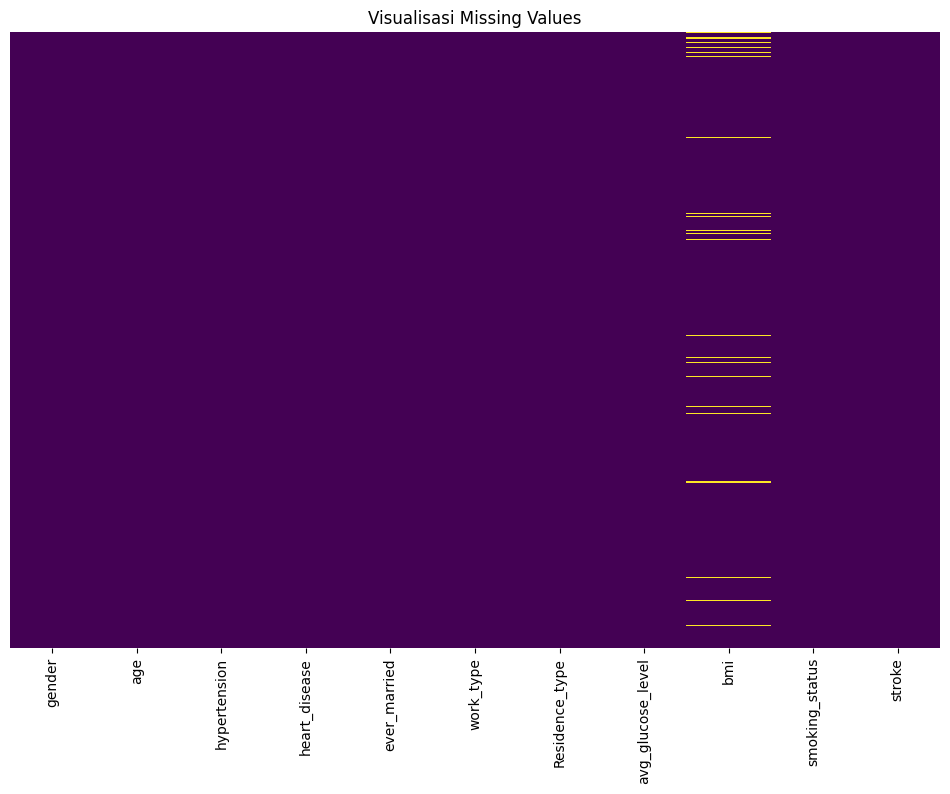
\includegraphics[width=\columnwidth]{./assets/missing-value.png}
        \caption{Distribusi Nilai Hilang pada Variabel BMI}%
        \label{fig:missing-value}
    \end{figure}

    \subsubsection{Feature Analysis}

    Tahap akhir preprocessing meliputi analisis mendalam terhadap hubungan
    antarvariabel melalui matriks korelasi yang ditampilkan pada Gambar
    \ref{fig:matrix-corelation}. Analisis korelasi ini memberikan pemahaman
    komprehensif tentang kekuatan dan arah hubungan antarvariabel dalam dataset.
    Nilai korelasi yang berkisar antara -1 hingga 1 mengindikasikan tingkat dan
    sifat hubungan antarvariabel, dengan nilai mendekati 1 atau -1 menunjukkan
    korelasi yang kuat dan nilai mendekati 0 menandakan hubungan yang lemah.

    \begin{figure}[H]
        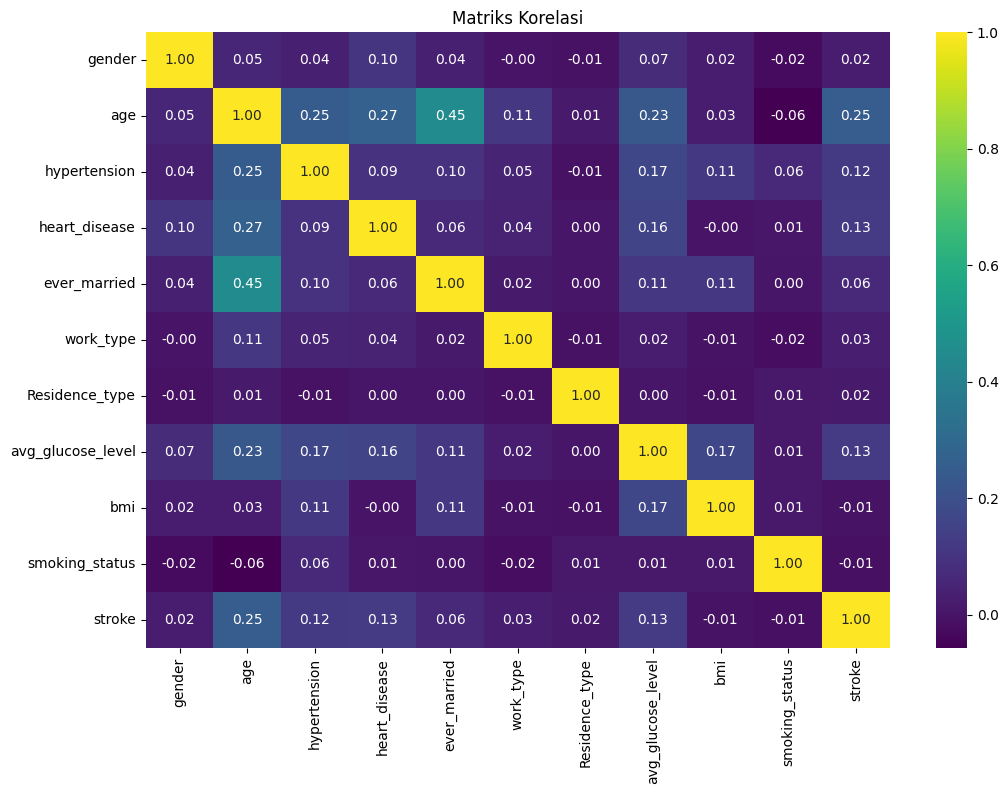
\includegraphics[width=\columnwidth]{./assets/matrix-corelation.png}
        \caption{Matriks Korelasi Variabel pada Dataset Stroke Prediction}%
        \label{fig:matrix-corelation}
    \end{figure}

    Hasil analisis matriks korelasi menunjukkan bahwa faktor usia memiliki korelasi
    tertinggi dengan kejadian stroke, yakni sebesar 0,25. Meskipun nilai ini
    tergolong rendah, temuan ini mengonfirmasi bahwa usia merupakan faktor yang
    paling berpengaruh dibandingkan dengan variabel lainnya. Rendahnya nilai
    korelasi secara keseluruhan mengindikasikan kompleksitas dalam memprediksi
    kejadian stroke dan menegaskan pentingnya pendekatan \textit{machine learning}
    yang mampu menangkap pola-pola kompleks dalam data. Temuan ini juga memperkuat
    pemahaman bahwa kelompok usia lanjut merupakan segmen populasi yang memerlukan
    perhatian khusus dalam upaya pencegahan stroke.

    \subsubsection{Outlier Analysis}

    Analisis outlier dilakukan untuk mengidentifikasi nilai-nilai ekstrem dalam
    dataset, khususnya pada variabel numerik seperti usia, BMI, dan level glukosa
    rata-rata, sebagaimana ditunjukkan pada Gambar \ref{fig:outliers-boxplot}.
    Meskipun terdeteksi beberapa nilai yang secara statistik dapat dikategorikan
    sebagai outlier, keputusan diambil untuk mempertahankan nilai-nilai tersebut
    dalam dataset. Pertimbangan ini didasarkan pada dua alasan utama: pertama,
    dalam konteks data medis, nilai-nilai ekstrem seringkali merepresentasikan
    kasus-kasus klinis yang valid dan penting; kedua, outlier tersebut dapat
    mengandung informasi yang bermakna tentang faktor risiko stroke, mengingat
    kondisi ekstrem seperti kadar glukosa yang sangat tinggi atau BMI yang jauh di
    atas normal memang berkorelasi dengan peningkatan risiko stroke.

    \begin{figure}[H]
        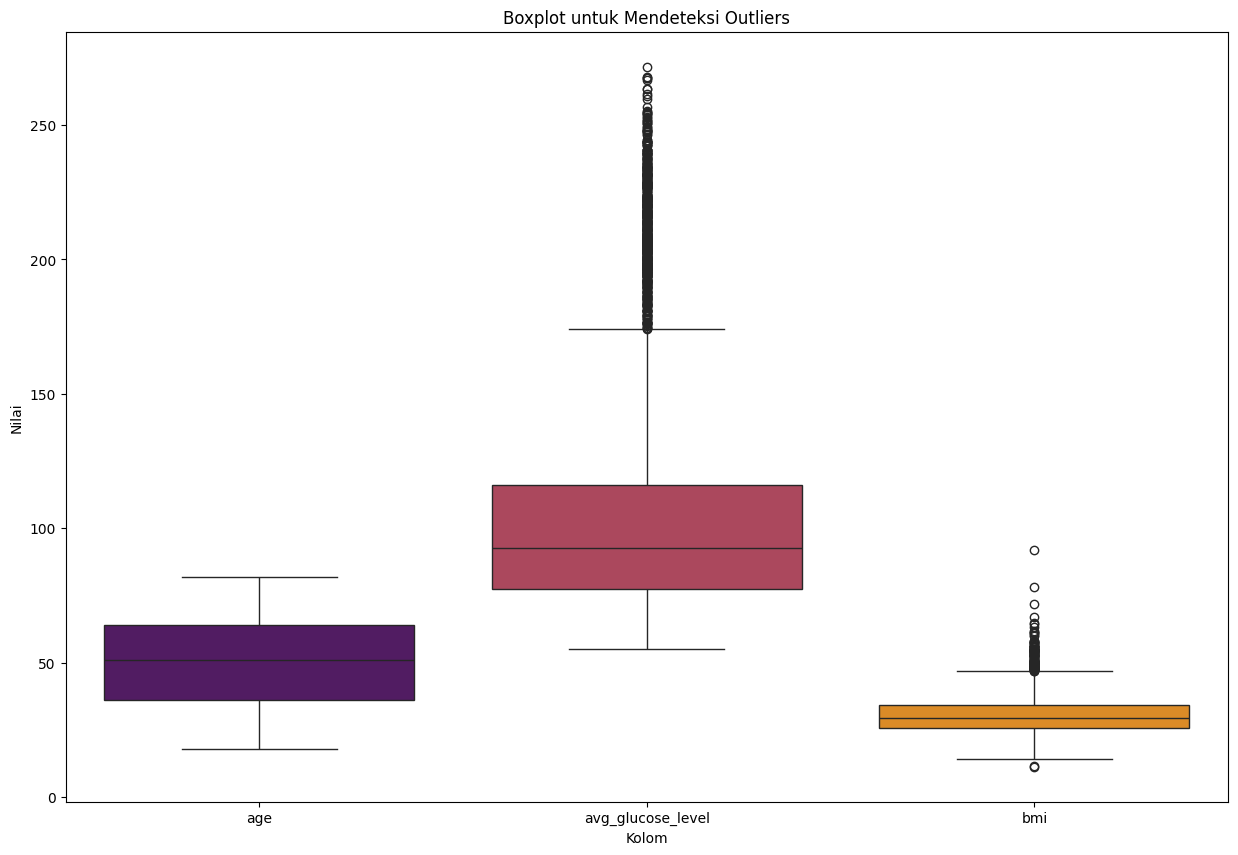
\includegraphics[width=\columnwidth]{./assets/outliers.png}
        \caption{Visualisasi Outlier pada Variabel Numerik}%
        \label{fig:outliers-boxplot}
    \end{figure}

    \subsubsection{Encoding}

    Sebelum data dapat diproses oleh algoritma \textit{machine learning}, seluruh
    variabel kategorikal dikonversi menjadi format numerik melalui proses Label
    Encoding. Metode ini diterapkan pada semua variabel kategorikal dalam dataset,
    termasuk \textit{gender}, \textit{ever\_married}, \textit{Residence\_type},
    \textit{work\_type}, dan \textit{smoking\_status}.

    Label Encoding mengonversi setiap kategori menjadi nilai numerik berurutan.
    Sebagai contoh, untuk variabel \textit{gender}, kategori ``Female'' dikonversi
    menjadi 0, ``Male'' menjadi 1, dan ``Other'' menjadi 2. Pendekatan serupa
    diterapkan pada variabel kategorikal lainnya, dengan setiap kategori unik
    diberikan nilai numerik yang berbeda. Meskipun pendekatan ini dapat
    menghasilkan asumsi ordinal implisit antarkategori, pemilihan Label Encoding
    untuk seluruh variabel kategorikal didasarkan pada pertimbangan efisiensi
    komputasi dan kesederhanaan model.

    Namun untuk kategori ``Other'' yang ada pada variabel gender, kami menghapusnya
    karena nilai tersebut sangat tidak relevan dan hanya terdapat pada satu sampel
    saja.

    \subsubsection{Data Splitting and K-Fold Cross Validation modified}

    Dataset dibagi menjadi beberapa subset menggunakan metode stratifikasi untuk
    memastikan distribusi kelas yang seimbang pada setiap bagian data. Setelah
    preprocessing, dataset akhir terdiri dari 247 kasus stroke dan 4006 kasus
    non-stroke. Pemisahan data ini dirancang khusus untuk mencegah kebocoran data
    sintetis ke dalam set pengujian yang dapat mengakibatkan overfitting dan bias
    pada estimasi performa model.

    \begin{table}[H]
        \centering
        \caption{Jumlah Data dalam Setiap Fold}
        \label{tab:data-splitting}
        \begin{tabular}{>{\raggedright\arraybackslash}p{2.5cm}>{\raggedright\arraybackslash}p{2cm}>{\raggedright\arraybackslash}p{2cm}}
            \specialrule{0.07em}{0em}{0.06em}
            \specialrule{0.07em}{0em}{0.4em}
            Fold   & Stroke & Non-Stroke \\
            \midrule
            Fold 1 & 49     & 801        \\
            Fold 2 & 49     & 801        \\
            Fold 3 & 49     & 801        \\
            Fold 4 & 50     & 801        \\
            Fold 5 & 50     & 802        \\
            \bottomrule
        \end{tabular}
    \end{table}

    Pembagian data untuk \textit{training} dan \textit{testing} dilakukan secara
    terpisah untuk kelas stroke dan non-stroke. Untuk kasus stroke, satu fold
    digunakan sebagai data \textit{testing} (sekitar 49-50 sampel), sementara empat
    fold lainnya digabungkan sebagai data \textit{training} (sekitar 197-198
    sampel). Sedangkan untuk kasus non-stroke, dari satu fold yang sama dengan
    \textit{testing} stroke, diambil 100 sampel secara acak sebagai data
    \textit{testing}, dan sisa data dalam fold tersebut (sekitar 701-702 sampel)
    digunakan sebagai data \textit{training}. Data non-stroke dari fold lainnya
    tidak digunakan dalam proses pemodelan untuk menghindari ketimpangan yang
    berlebihan dalam data \textit{training}.

    Proses validasi dilakukan dengan melakukan iterasi sebanyak 25 kali yang
    merupakan kombinasi dari 5 fold stroke dan 5 fold non-stroke yang berbeda.
    Setiap iterasi menggunakan kombinasi fold yang unik untuk memastikan evaluasi
    yang komprehensif terhadap performa model. Rincian kombinasi fold dan komposisi
    data untuk setiap iterasi dapat dilihat pada Tabel \ref{tab:fold-combinations}.

    \subsubsection{Data Balancing}
    Untuk mengatasi ketidakseimbangan data yang signifikan antara kelas stroke
    (minoritas) dan non-stroke (mayoritas), penelitian ini menerapkan teknik SMOTE
    (Synthetic Minority Over-sampling Technique). SMOTE bekerja dengan menciptakan
    sampel sintetis dari kelas minoritas untuk menyeimbangkan distribusi kelas.
    Proses ini dilakukan secara sistematis dengan menggunakan interpolasi antara
    sampel-sampel kelas minoritas yang berdekatan dalam ruang fitur.

    SMOTE menghasilkan sampel sintetis dengan mencari K tetangga terdekat dari
    kelas yang sama menggunakan jarak Euclidean, memilih secara acak salah satu
    dari K tetangga terdekat, menghitung vektor perbedaan, dan menghasilkan sampel
    sintetis menggunakan rumus $x_{new} = x_i + \lambda\delta$, dengan $\lambda$
    adalah bilangan acak antara 0 dan 1.

    Dalam implementasinya, SMOTE diterapkan hanya pada data \textit{training} untuk
    menghindari kebocoran data. Parameter yang digunakan adalah rasio oversampling
    0.7 untuk meminimalisir risiko overfitting, jumlah tetangga terdekat 5, dan
    random state 42.

    Setelah penerapan SMOTE, distribusi kelas dalam data \textit{training} menjadi
    lebih seimbang, membantu model dalam mempelajari pola dari kedua kelas secara
    lebih efektif. Penting untuk dicatat bahwa data \textit{testing} tetap
    mempertahankan distribusi aslinya untuk memastikan evaluasi yang realistis
    terhadap performa model.

    \begin{figure}[H]
        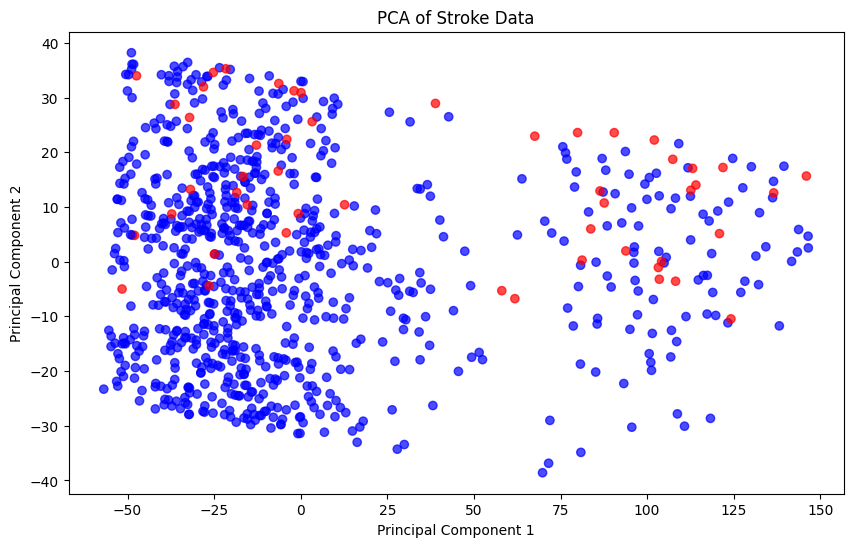
\includegraphics[width=\columnwidth]{./assets/before-smote.png}
        \caption{Distribusi Kelas Sebelum Penerapan SMOTE pada Data \textit{training}}%
        \label{fig:class-distribution-before-smote}
    \end{figure}
    \begin{figure}[H]
        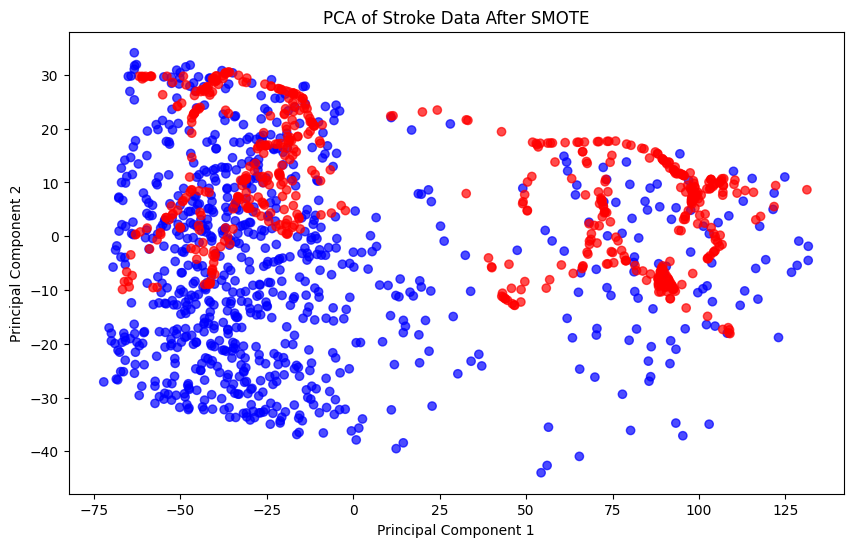
\includegraphics[width=\columnwidth]{./assets/after-smote.png}
        \caption{Distribusi Kelas Setelah Penerapan SMOTE pada Data \textit{training}}%
        \label{fig:class-distribution-after-smote}
    \end{figure}

\end{multicols}

\begin{landscape}
\begin{table}[htbp]
    \centering
    \caption{Kombinasi Fold dan Komposisi Data pada Setiap Iterasi}%
    \label{tab:fold-combinations}
    \begin{tabular}{>{\raggedright\arraybackslash}p{2cm} >{\raggedright\arraybackslash}p{2cm} >{\raggedright\arraybackslash}p{2cm} >{\raggedright\arraybackslash}p{2cm} >{\raggedright\arraybackslash}p{2cm} >{\raggedright\arraybackslash}p{2cm} >{\raggedright\arraybackslash}p{2cm} >{\raggedright\arraybackslash}p{2cm} >{\raggedright\arraybackslash}p{2cm}}
        \specialrule{0.07em}{0em}{0.06em}
        \specialrule{0.07em}{0em}{0.4em}
        \multirow{2}{*}{Iterasi} & \multicolumn{2}{c}{Testing Fold} & \multicolumn{2}{c}{Data Testing} & \multicolumn{2}{c}{Data Training} & \multicolumn{2}{c}{Data Training with SMOTE} \\
        \cmidrule(lr){2-3} \cmidrule(lr){4-5} \cmidrule(lr){6-7} \cmidrule(lr){8-9}
                                 & Stroke                           & Non-stroke                       & Stroke                            & Non-stroke & Stroke & Non-stroke & Stroke & Non-stroke \\
        \midrule
        1                        & S1                               & N1                               & 49                                & 100        & 198    & 701        & 491    & 701  \\
        2                        & S1                               & N2                               & 49                                & 100        & 198    & 701        & 491    & 701  \\
        3                        & S1                               & N3                               & 49                                & 100        & 198    & 701        & 491    & 701  \\
        4                        & S1                               & N4                               & 49                                & 100        & 198    & 701        & 491    & 701  \\
        5                        & S1                               & N5                               & 49                                & 100        & 198    & 702        & 491    & 702  \\
        6                        & S2                               & N1                               & 49                                & 100        & 198    & 701        & 491    & 701  \\
        7                        & S2                               & N2                               & 49                                & 100        & 198    & 701        & 491    & 701  \\
        8                        & S2                               & N3                               & 49                                & 100        & 198    & 701        & 491    & 701  \\
        9                        & S2                               & N4                               & 49                                & 100        & 198    & 701        & 491    & 701  \\
        10                       & S2                               & N5                               & 49                                & 100        & 198    & 702        & 491    & 702  \\
        11                       & S3                               & N1                               & 49                                & 100        & 198    & 701        & 491    & 701  \\
        12                       & S3                               & N2                               & 49                                & 100        & 198    & 701        & 491    & 701  \\
        13                       & S3                               & N3                               & 49                                & 100        & 198    & 701        & 491    & 701  \\
        14                       & S3                               & N4                               & 49                                & 100        & 198    & 701        & 491    & 701  \\
        15                       & S3                               & N5                               & 49                                & 100        & 198    & 702        & 491    & 702  \\
        16                       & S4                               & N1                               & 50                                & 100        & 197    & 701        & 490    & 701  \\
        17                       & S4                               & N2                               & 50                                & 100        & 197    & 701        & 490    & 701  \\
        18                       & S4                               & N3                               & 50                                & 100        & 197    & 701        & 490    & 701  \\
        19                       & S4                               & N4                               & 50                                & 100        & 197    & 701        & 490    & 701  \\
        20                       & S4                               & N5                               & 50                                & 100        & 197    & 702        & 490    & 702  \\
        21                       & S5                               & N1                               & 50                                & 100        & 197    & 701        & 490    & 701  \\
        22                       & S5                               & N2                               & 50                                & 100        & 197    & 701        & 490    & 701  \\
        23                       & S5                               & N3                               & 50                                & 100        & 197    & 701        & 490    & 701  \\
        24                       & S5                               & N4                               & 50                                & 100        & 197    & 701        & 490    & 701  \\
        25                       & S5                               & N5                               & 50                                & 100        & 197    & 702        & 490    & 702  \\
        \bottomrule
    \end{tabular}
\end{table}
\end{landscape}

\begin{multicols}{2}
    \setlength{\columnsep}{0.4pt} %
    \raggedcolumns%
    \sloppy

    \subsection{Machine Learning Classification Methods}
    Pengembangan model prediksi stroke dalam penelitian ini menggunakan dua
    algoritma \textit{machine learning} yang berbeda, yaitu Random Forest dan
    Support Vector Machine. Pemilihan kedua algoritma ini didasarkan pada
    keunggulan masing-masing dalam menangani data medis yang kompleks serta
    kemampuannya dalam menghasilkan model prediksi yang akurat dan
    interpretabel\cite{zhang2023random}.

    \subsubsection{Random Forest}
    Random Forest merupakan algoritma \textit{machine learning} ensemble yang
    mengombinasikan kekuatan dari multiple pohon keputusan untuk menghasilkan
    prediksi yang lebih akurat dan stabil\cite{zhang2023random}. Algoritma ini
    dipilih karena beberapa keunggulan: (1) kemampuannya menangani data dengan
    dimensi tinggi, (2) ketahanannya terhadap overfitting, dan (3) kemampuannya
    memberikan informasi tentang pentingnya setiap fitur dalam proses prediksi.
    Setiap pohon keputusan dalam Random Forest dibangun menggunakan subset acak
    dari data pelatihan melalui teknik bootstrap aggregating (bagging), yang
    meningkatkan variasi antar pohon dan mengurangi variance prediksi akhir.

    Random Forest merupakan algoritma \textit{machine learning} ensemble yang
    terdiri atas kumpulan pohon keputusan. Setiap pohon keputusan dibangun
    menggunakan subset acak dari data pelatihan melalui teknik bootstrap
    aggregating (bagging). Untuk suatu dataset dengan n sampel dan m fitur, Random
    Forest menggunakan formula berikut untuk membangun setiap pohon:

    \begin{equation}
        f_{RF}(x) = \frac{1}{B}\sum_{b=1}^{B}T_b(x)
    \end{equation}

    dengan $f_{RF}(x)$ adalah prediksi akhir Random Forest, B adalah jumlah pohon,
    dan $T_b(x)$ adalah prediksi dari pohon ke-b. Setiap pohon dibangun dengan
    mempertimbangkan subset fitur $m_{try}$ yang dipilih secara acak, dengan:

    \begin{equation}
        m_{try} = \lfloor\sqrt{m}\rfloor
    \end{equation}

    Pemilihan fitur pada setiap node menggunakan kriteria Gini Impurity:

    \begin{equation}
        Gini(t) = 1 - \sum_{i=1}^{c}p(i|t)^2
    \end{equation}

    dengan $p(i|t)$ adalah proporsi kelas i pada node t, dan c adalah jumlah kelas.

    Dalam implementasinya, ruang pencarian hiperparameter Random Forest mencakup
    beberapa parameter kunci: jumlah pohon (\texttt{n\_estimators}) dengan rentang
    10 hingga 200, kedalaman maksimum pohon (\texttt{max\_depth}) dari 1 hingga 50,
    jumlah minimum sampel untuk pemisahan internal (\texttt{min\_samples\_split})
    dari 2 hingga 20, jumlah minimum sampel pada setiap daun
    (\texttt{min\_samples\_leaf}) dari 1 hingga 20, dan proporsi fitur yang
    digunakan (\texttt{max\_features}) dengan rentang 0,1 hingga 1,0 yang
    didistribusikan secara seragam.

    \subsubsection{Support Vector Machine}
    Support Vector Machine (SVM) dipilih karena kemampuannya yang telah terbukti
    dalam berbagai aplikasi medis, khususnya dalam prediksi
    penyakit\cite{pisner2020support}. Dalam penelitian ini, digunakan SVM linear
    yang bekerja dengan mencari hyperplane optimal yang memaksimalkan margin
    pemisahan antara kelas stroke dan non-stroke. Menurut kajian
    terbaru\cite{bhavsar2021comprehensive}, pemilihan SVM linear memiliki
    keunggulan dalam hal interpretabilitas model dan efisiensi komputasi, terutama
    untuk dataset medis dengan fitur yang telah diseleksi dengan baik.

    Support Vector Machine linear bekerja dengan mencari hyperplane optimal yang
    memisahkan data ke dalam dua kelas. Fungsi objektif SVM linear dapat
    diformulasikan sebagai berikut:

    \begin{equation}
        \min_{\mathbf{w},b,\xi} \frac{1}{2}\|\mathbf{w}\|^2 + C\sum_{i=1}^{n}\xi_i
    \end{equation}

    dengan kendala:
    \begin{equation}
        y_i(\mathbf{w}^T\mathbf{x}_i + b) \geq 1 - \xi_i, \quad \xi_i \geq 0
    \end{equation}

    Dalam persamaan tersebut, $\mathbf{w}$ merupakan vektor bobot yang menentukan
    orientasi hyperplane, $b$ adalah bias, $\xi_i$ merupakan variabel slack yang
    memungkinkan kesalahan klasifikasi, dan $C$ merupakan parameter regularisasi
    yang mengontrol keseimbangan antara margin maksimum dan error klasifikasi.

    Ruang pencarian hiperparameter SVM meliputi parameter regularisasi $C$ dengan
    rentang dari $10^{-6}$ hingga $10^{6}$ yang didistribusikan secara log-uniform,
    parameter \texttt{gamma} untuk kernel RBF dengan rentang dari $10^{-6}$ hingga
    $10^{1}$ yang juga didistribusikan secara log-uniform, serta penggunaan kernel
    RBF yang telah ditetapkan. Distribusi log-uniform dipilih untuk parameter $C$
    dan \texttt{gamma} karena rentang nilai yang mencakup beberapa tingkat besaran,
    memungkinkan eksplorasi yang lebih efektif pada skala logaritmik.

    \subsection{Model Optimization}

    Optimasi model dilaksanakan menggunakan Optimasi Bayesian, suatu pendekatan
    optimasi berurutan yang memanfaatkan model probabilistik untuk memetakan fungsi
    objektif dan menentukan parameter optimal. Dalam penelitian ini, fungsi
    objektif yang dimaksud adalah nilai F1-score yang dihasilkan model sebagai
    fungsi dari kombinasi hiperparameter yang digunakan.

    Optimasi Bayesian menerapkan dua komponen utama dalam prosesnya. Komponen
    pertama adalah model pengganti (\textit{surrogate model}) yang menggunakan
    Gaussian Process untuk memetakan hubungan antara hiperparameter dan performa
    model. Komponen kedua adalah fungsi akuisisi yang menentukan titik evaluasi
    berikutnya dengan menyeimbangkan antara eksplorasi ruang parameter yang belum
    dijelajahi dan eksploitasi area yang menunjukkan hasil menjanjikan.

    Proses optimasi dilaksanakan secara sistematis dan berurutan. Diawali dengan
    pembangunan model probabilistik berdasarkan data hasil evaluasi sebelumnya,
    dilanjutkan dengan penentuan titik evaluasi berikutnya menggunakan fungsi
    akuisisi. Setelah itu, dilakukan evaluasi pada kombinasi parameter yang
    dipilih, dan model probabilistik diperbarui dengan hasil evaluasi terbaru.
    Proses ini diulang hingga mencapai jumlah iterasi yang telah ditetapkan.

    Implementasi optimasi menggunakan BayesSearchCV dengan pengaturan yang telah
    disesuaikan untuk kasus ini. Jumlah iterasi pencarian ditetapkan sebanyak 32
    kali, dengan setiap iterasi mengevaluasi kombinasi hiperparameter yang berbeda.
    \textit{cross validation} menggunakan 3-lipatan untuk memperoleh estimasi
    performa yang lebih andal. Untuk memastikan hasil yang dapat direproduksi,
    nilai \texttt{random\_state} ditetapkan pada 42, sementara penggunaan sumber
    daya komputasi dioptimalkan dengan mengatur \texttt{n\_jobs} ke -1.

    Pendekatan ini menghasilkan proses pencarian hiperparameter yang lebih efisien
    dibandingkan dengan metode Grid Search atau Random Search konvensional.
    Keunggulan ini diperoleh karena kemampuannya memanfaatkan informasi dari
    evaluasi sebelumnya untuk mengarahkan pencarian ke area yang lebih menjanjikan,
    sehingga menghasilkan kombinasi parameter yang optimal dengan lebih cepat dan
    efektif.

    \subsection{Performance Metrics}
    Dalam evaluasi model klasifikasi stroke, kami menggunakan beberapa metrik
    performa standar yang diperoleh dari \textit{confusion matrix}.

    Accuracy mengukur proporsi total prediksi yang benar dibandingkan dengan semua
    kasus.
    \begin{equation}
        Accuracy = \frac{TP + TN}{TP + TN + FP + FN}
    \end{equation}

    Precision mengukur proporsi prediksi positif yang benar-benar positif.
    \begin{equation}
        Precision = \frac{TP}{TP + FP}
    \end{equation}

    Recall (Sensitivity) mengukur proporsi kasus positif yang berhasil
    diidentifikasi.
    \begin{equation}
        Recall = \frac{TP}{TP + FN}
    \end{equation}

    F1-Score merupakan rata-rata harmonik dari \textit{precision} dan
    \textit{recall}.
    \begin{equation}
        \text{F1-Score} = \frac{2 \times \text{Precision} \times \text{Recall}}{\text{Precision} + \text{Recall}}
    \end{equation}

    Dalam konteks ini, TP (\textit{True Positive}) adalah jumlah kasus stroke yang
    diprediksi benar sebagai stroke. TN (\textit{True Negative}) merupakan jumlah
    kasus non-stroke yang diprediksi benar sebagai non-stroke. FP (\textit{False
        Positive}) menunjukkan jumlah kasus non-stroke yang salah diprediksi sebagai
    stroke. FN (\textit{False Negative}) adalah jumlah kasus stroke yang salah
    diprediksi sebagai non-stroke.

    Pemilihan metrik-metrik ini didasarkan pada karakteristik dataset yang tidak
    seimbang, sehingga F1-score menjadi sangat penting karena memberikan gambaran
    yang lebih baik tentang performa model pada kasus yang tidak seimbang
    dibandingkan dengan \textit{accuracy} saja.\@ \textit{Recall} juga penting
    dalam kasus prediksi stroke karena fokus utama adalah pada identifikasi kasus
    positif (stroke) yang sebenarnya.

    \subsection{Modified K-Fold Cross Validation}
    Untuk mengatasi ketidakseimbangan data dan memastikan evaluasi model yang
    akurat, penelitian ini menggunakan validasi silang K-Fold yang dimodifikasi.
    Teknik ini membagi dataset menjadi K subset dengan distribusi kelas yang
    seimbang di setiap fold, sehingga performa model pada kelas minoritas dapat
    dievaluasi secara lebih representatif.

    \section{Results and Discussion}
    Hasil dari validasi silang K-Fold yang dimodifikasi menunjukkan bahwa model SVM
    dengan SMOTE dan Optimasi Bayesian mencapai performa tertinggi secara konsisten
    di seluruh fold, mengindikasikan kemampuan generalisasi yang baik.

    % Example of single-column figure

    % Use table* to span both columns

    % \begin{multicols}{2}
    % Results and discussion content goes here...

    \section{Conclusion}
    Penerapan validasi silang K-Fold yang dimodifikasi terbukti efektif dalam
    evaluasi model pada dataset yang tidak seimbang, meningkatkan akurasi dan
    keandalan prediksi risiko stroke.

    \section*{Acknowledgements}
    % Acknowledgements content goes here...

    \bibliography{references}

\end{multicols}
\end{document}
